
%What do we want to test?

%Short term model:
%- the event specification; 
%        - new data: Bloomberg global
%        - requiring 2/3 SDs for the event rule
%        - mkt cap vs. value weighted. 

%Long term:
%- mkt cap vs. value weighted. 
%- Developed market factors


In this section I will examine the robustness of the results by altering the model variables or event requirements and re-estimate the results, as it is important to cross-validate that a potential appearance of over-performance is not created artificially. Thus, the practice can lead to validation or invalidation along with advancement of model specifications. 

\subsection{Market model: event specification}
The requirement rule for event identification is based on the magnitude of events in relation to the average event for the individual firm. Thus, it seems plausible that an increase in the tightness of the requirement rule will lead to higher abnormal returns in absolute values.  
To address the issue I test whether the short term abnormal returns are sensitive to the methodology in specifying individual events. Specifically, I re-estimate the models with a requirement stating that the events should be more than, respectively, two and three standard deviations from the average event. A tighter event specification determine that fewer stocks will be included in the model as less events will be regarded as important. Consequently, the events included should be more negative or positive with a stricter rule. 

The results are reported in table \ref{tab: ST_significace}, which demonstrate that negative events continue to generate significant abnormal returns, while positive events does not. Due to insignificance and borderline randomness of the relation between positive events and returns I will only present the plots related to negative events. The graph of the positive events can be found in Appendix \ref{fig:ST_pos_sensi}. 


\begin{table}[ht]
\centering
\caption{AAR and CAAR (in \%) with new event rule (sd)} 
\begin{tabular}{lccccc}
  \hline  \hline
  & \multicolumn{2}{c}{Positive} &  & \multicolumn{2}{c}{Negative}\\ \cline{2-3} \cline{5-6}  
  & 2 sd & 3 sd & & 2 sd & 3 sd   \\   
 \hline
$AAR_{t=0}$ & $\underset{(0.875)}{0.051}$ & $\underset{(-0.278)}{-0.022}$ & & $\underset{(-3.409)}{-0.522^{***}}$ & $\underset{(-3.024)}{-0.617^{***}}$ \\ 
$CAAR_{[-2;+2]}$  & $\underset{(0.283)}{0.031}$  & $\underset{(0.631)}{0.089}$ & & $\underset{(-3.66)}{-0.714^{***}}$ & $\underset{(-2.648)}{-0.657^{***}}$ \\ 
$CAAR_{[-5;+5]}$  & $\underset{(1.197)}{0.195}$  & $\underset{(1.350)}{0.290}$ & &$\underset{(-3.56)}{-0.902^{***}}$ & $\underset{(-2.782)}{-0.867^{***}}$ \\ 
$CAAR_{[-10;+10]}$  & $\underset{(-0.168)}{-0.035}$  & $\underset{(-0.062)}{-0.018}$ &  & $\underset{(-1.886)}{-0.652^{*}}$ & $\underset{(-1.686)}{-0.697^{*}}$ \\ 
N & 1845 & 1078 & & 648 & 451  \\
   \hline \hline
   \multicolumn{6}{p{12cm}}{ \footnotesize $^* \; p\; <\; 0.1$, $ ^{**} \; p\; <\; 0.05$, $ ^{***} \; p\; <\; 0.01$  } \\
   \multicolumn{6}{p{13cm}}{\footnotesize The table shows the CAAR associated with positive and negative news over an event window of 5, 10, and 21 days surrounding the event date along with the AAR on $t=0$. The models are split on the requirement rule for included events (2 or 3 sd).} \\
   \hline
\end{tabular}
\label{tab:ST_sensitivity}
\end{table}

The two new models based on negative events are compared to the original results (1 sd) in figure \ref{fig:ST_neg_sensitivity}. The AAR is presented in dotted lines and the CAAR in solid lines along with estimation requirements of 1 sd (red), 2 sd (green), and 3 sd (blue). For simplicity, I have skipped the confidence intervals along with the barchart, which represented the relative amount of events. The similarities of the AAR and CAAR imply that the results are robust to changes in the event specification. While it is clear that enforcing a stronger sd requirement leads to lower AARs on the event date, no effect on the CAAR is present, visually, over the full event window. From table \ref{tab:ST_sensitivity}, the AAR on $t=0$ is, respectively, -0.52\% and -0.61\% for the 2 and 3 sd requirements compared to -0.37\% for the original 1 sd, meaning that the greatest instantaneous causal impact happens with a tight event rule. All are significant on the 1\% level. Intuitively, the investor reaction is more severe when events are identified as more important.  


\begin{figure} [h]
    \centering
    \caption{Negative news: Update event requirement}
    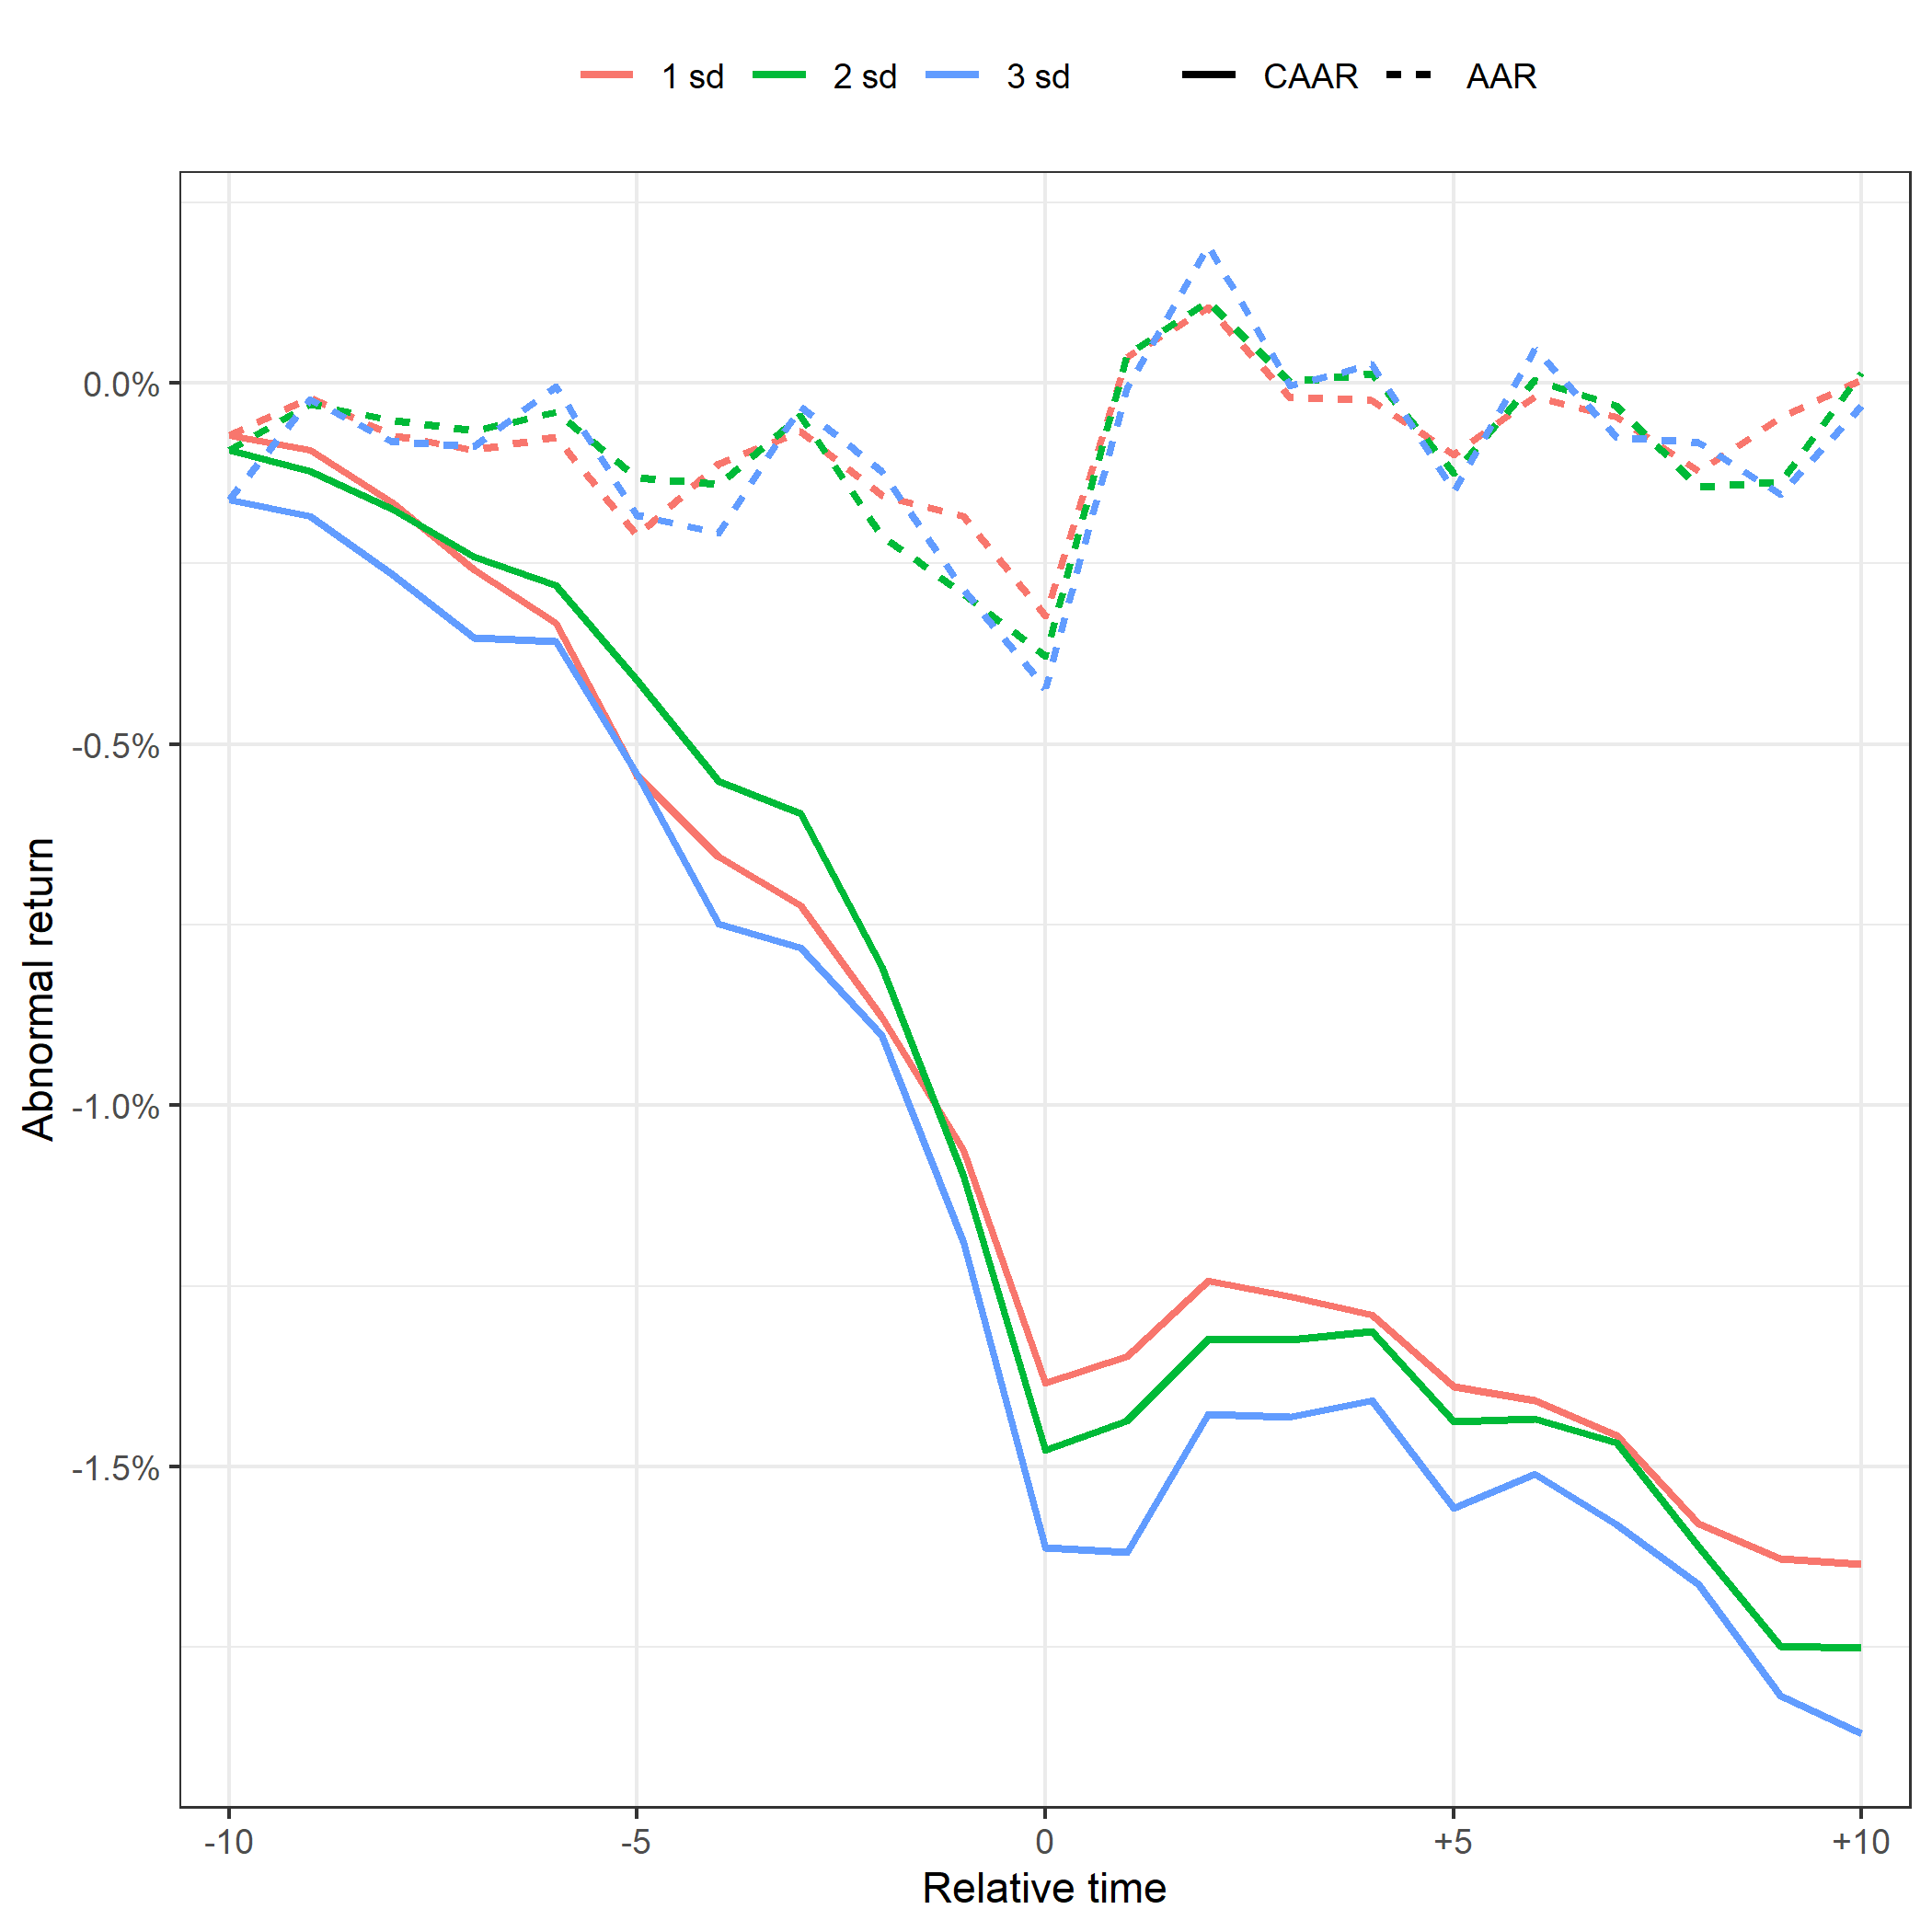
\includegraphics[scale=0.6]{Projekt/1.Figures analysis/ST_negative_sensitivity.png}
     \caption*{\footnotesize The figure illustrates the average abnormal return (AAR) and cumulative AAR (CAAR) around the event date (t = 0) of negative news. The various colors represent whether the event identification rule was based on 1, 2, or 3 standard errors.  }
    \label{fig:ST_neg_sensitivity}
\end{figure} 



\subsection{Market model: value vs. equal weights}

A portfolio of stocks needs to be weighted in order to determine the relative impact the individual constituents have on the performance of the portfolio. Throughout the paper the portfolio weights have been based on the relative market capitalization of the firms - also known as value weights. Table \ref{tab:ST_sensitivity_weights} compares the performance of the value weighted portfolio against an equal weighted. The portfolios hold the same firms, however with different weights, and are based on the same identified events. Again, the results from using equal weights show that none of the portfolio returns, associated with positive events, are significant. 

The equal weighted portfolio returns associated with negative events the empirical results from the former section is more or less valid. As expected, the returns are slightly different. However, they do appear significant on the same level and with the same direction of returns as the original results. While the portfolio AARs apparently follow each other to some extent, the development in CAAR is more adverse using equal weights relative to value weights. A potential explanation is that an equal weighted portfolio will award more weight to small stocks, thus they will contribute more to the portfolio returns relative to an value weighted portfolio. As small stocks tends to be more volatile than larger stocks \cite{Fama_french_3fac}, negative news could drive portfolio returns lower. 

In the period following a given event, the average reaction from equal and value weighted portfolios are different. Although the AARs at this point are insignificant, the CAAR series indicate that the equal weighted portfolio, which favor small stocks, is pricing in events in the days following an actual event, whereas most of the negative price action is happening before the event has occurred for the value weighted portfolio. Possibly, news about small stocks will take time to reach a large amount of investors, which is why the price reaction is happening at a later point. 

\begin{figure} [H]
    \centering
    \caption{Negative news: Value vs. Equal weights}
    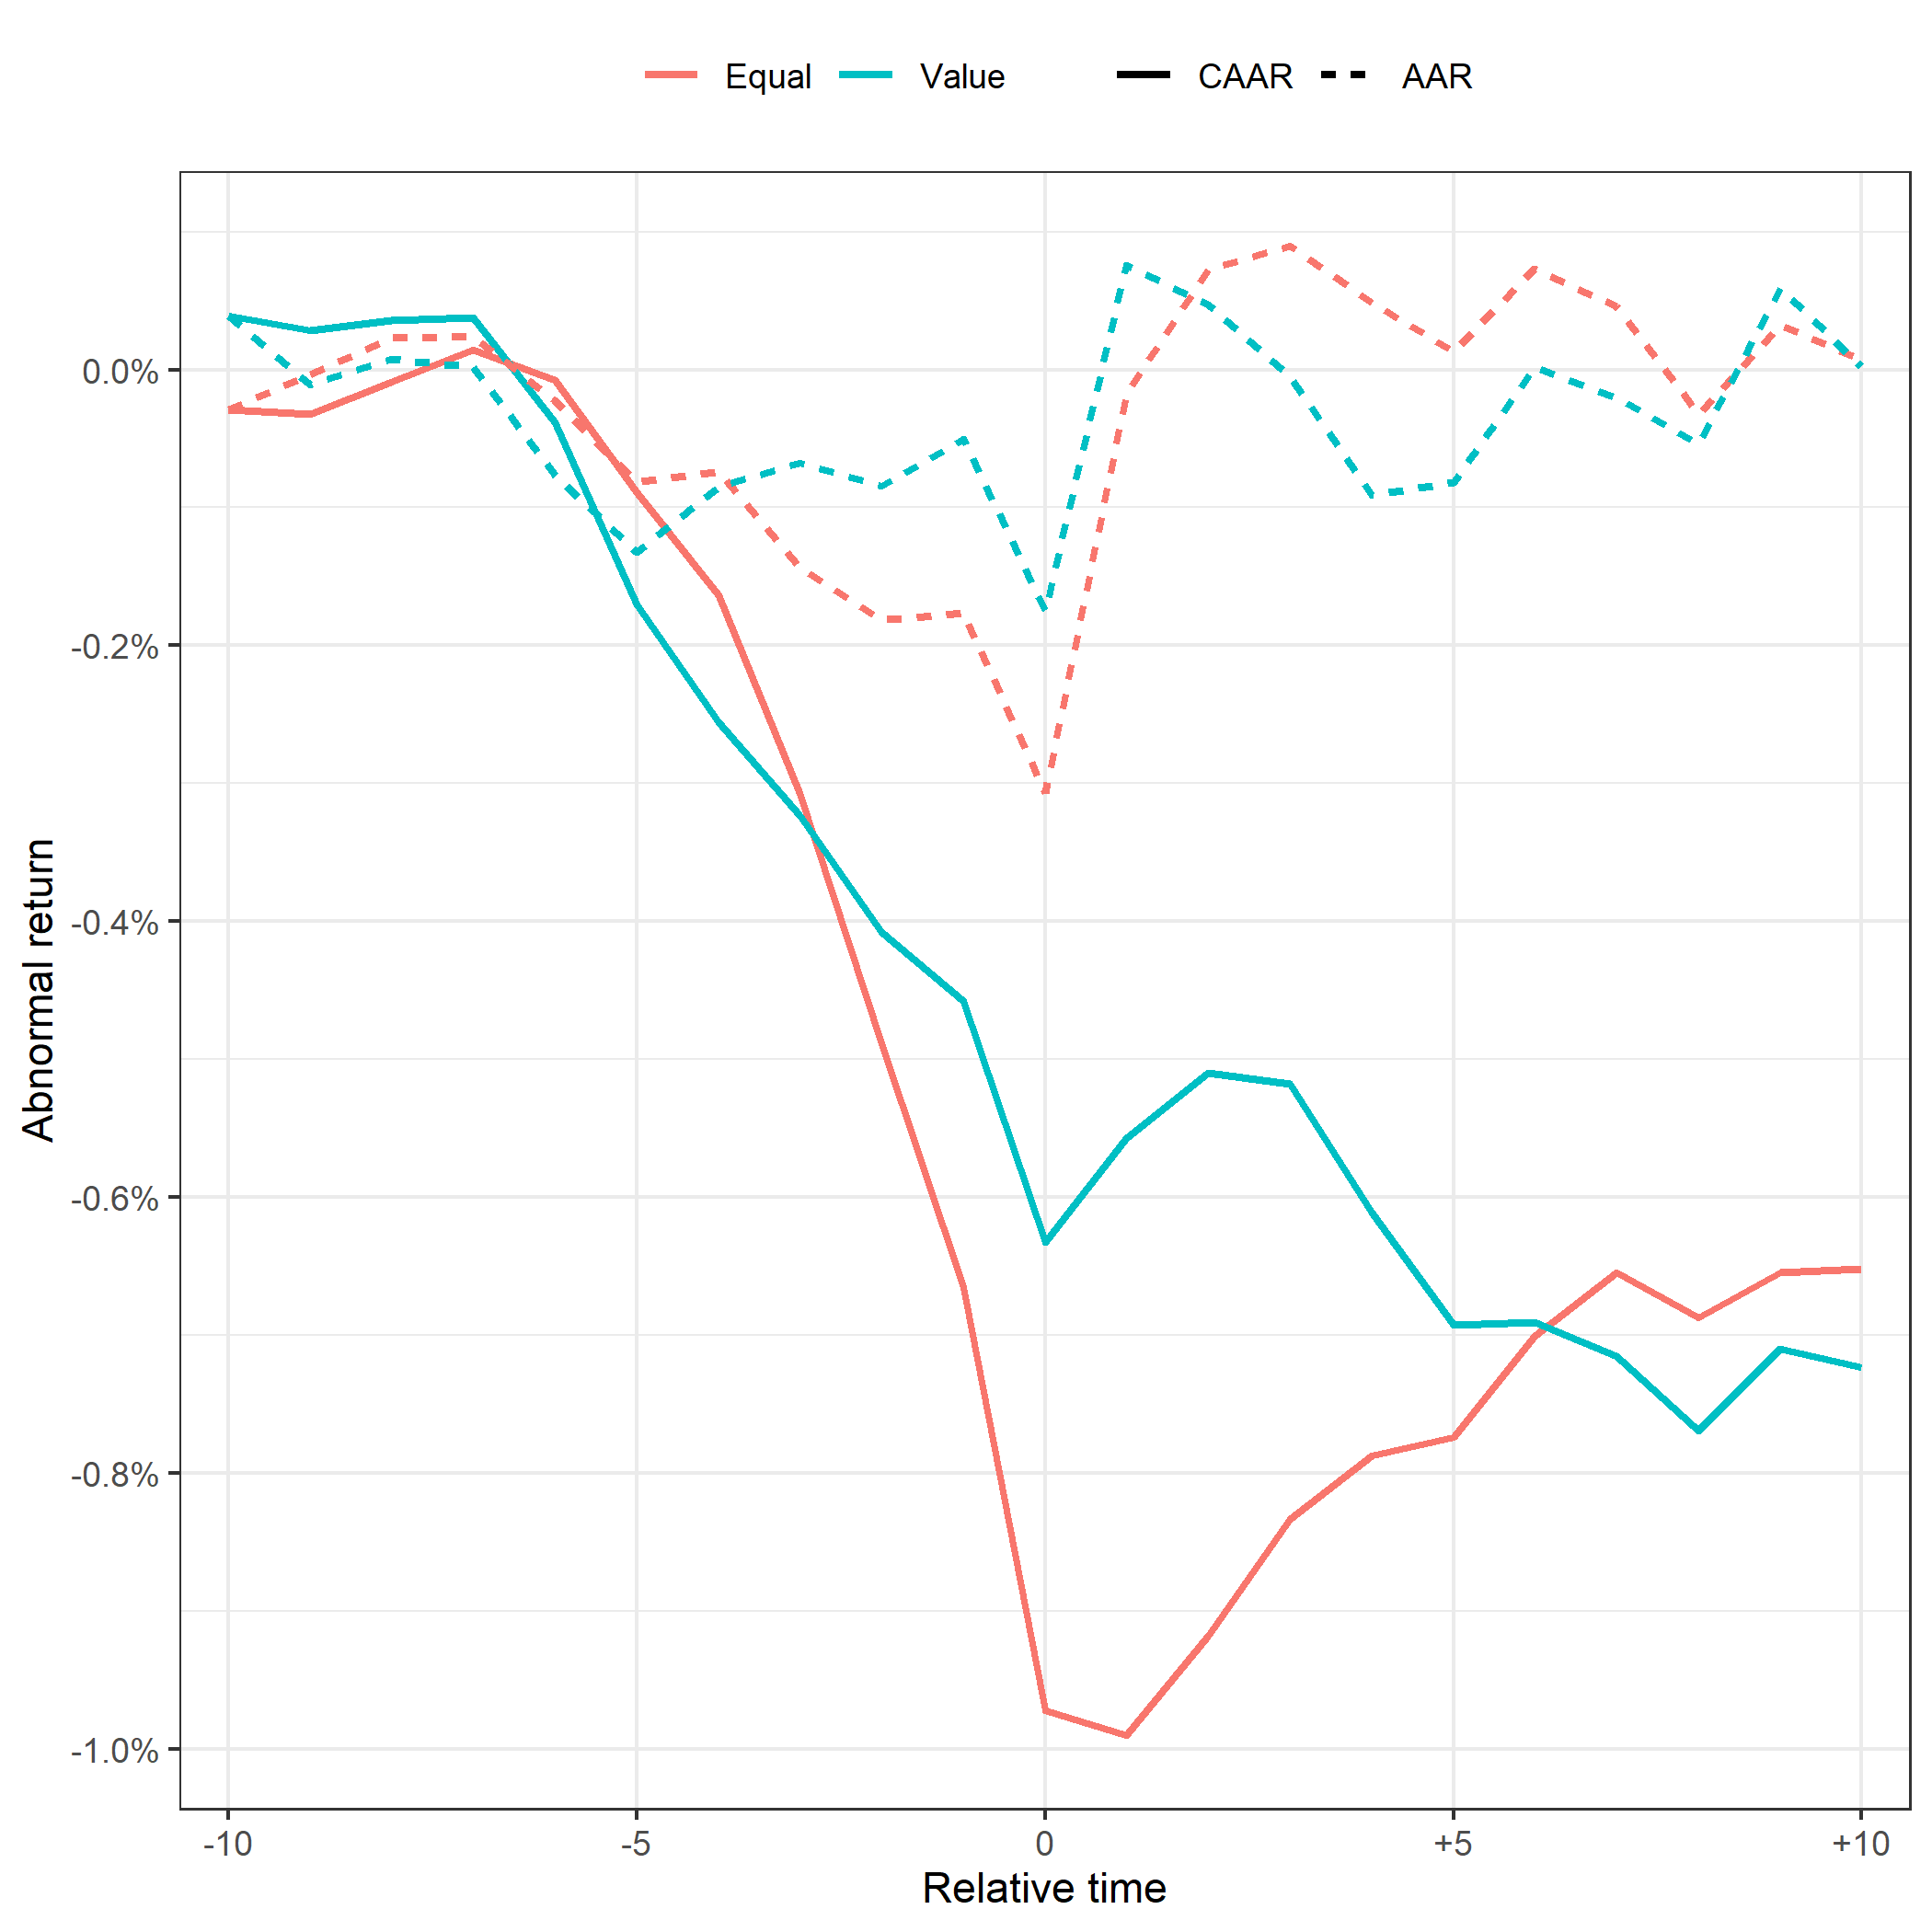
\includegraphics[scale=0.6]{Projekt/1.Figures analysis/ST_negative_sensitivity_weight.png}
     \caption*{\footnotesize The figure illustrates the average abnormal return (AAR) and cumulative AAR (CAAR) around the event date (t = 0) of negative news. The blue lines are returns calculated from an equally weighted portfolio, while the weights of the red lines are based on market capitalization.}
    \label{fig:ST_neg_sensitivity_weight}
\end{figure} 


\begin{table}[ht]
\centering
\caption{AAR and CAAR (in \%) with equally weighted returns} 
\begin{tabular}{lcccc}
  \hline  \hline
  & \multicolumn{1}{c}{Positive} &  \multicolumn{1}{c}{Negative}\\  
 \hline
$AAR_{t=0}$ &  $\underset{(0.634)}{0.045}$ & $\underset{(-3.509)}{-0.400^{***}}$ \\ 
$CAAR_{[-2;+2]}$  & $\underset{(0.367)}{0.053}$ & $\underset{(-4.120)}{-0.662^{***}}$ \\ 
$CAAR_{[-5;+5]}$  & $\underset{(-1.233)}{-0.258}$ & $\underset{(-5.457)}{-1.100^{***}}$ \\ 
$CAAR_{[-10;+10]}$    & $\underset{(-0.452)}{-0.128 }$ & $\underset{(-5.702)}{-1.558^{***}}$ \\ 
   \hline \hline
   \multicolumn{3}{p{10cm}}{ \footnotesize $^* \; p\; <\; 0.1$, $ ^{**} \; p\; <\; 0.05$, $ ^{***} \; p\; <\; 0.01$  } \\
   \multicolumn{3}{p{10cm}}{\footnotesize The tables shows the CAAR associated with positive and negative news over an event window of 5, 10, and 21 days surrounding the event date along with the AAR on $t=0$. The models are split on the requirement rule for included events (2 or 3 sd).} \\
   \hline
\end{tabular}
\label{tab:ST_sensitivity_weights}
\end{table}







\subsection{Calendar Time Portfolio: Portfolio weights}

\setlength{\tabcolsep}{15pt}
\begin{table}[]
\small
\centering
\caption{Fama-French five-factor model alpha from negative news with equal weights} 
\begin{tabular}{ccccccc}
\hline \hline \\ 
 &     &  &    1 SD  &  2 SD  &  3 SD  &  \\ \cline{4-6} 
& & & \multicolumn{3}{c}{ T = 1} & \\ \cline{2-6}
& Alpha (\%)  &  & $-0.96^{***}$  & $-0.94^{***}$  & $-0.90^{**}$ &  \\
& t-value &  & -3.94 & -2.87  & -1.92 & \\
& & & \multicolumn{3}{c}{ T = 4} & \\ \cline{2-6}
& Alpha (\%)  &  & $-0.70^{***}$  & $-0.84^{***}$  &  $-0.81^{***}$ & \\
& t-value & & -3.95 & -4.28 & -2.99 & \\
& & & \multicolumn{3}{c}{ T = 8} & \\ \cline{2-6}
& Alpha (\%)  &  & $-0.64^{***}$   & $-0.67^{***}$  & $-0.73^{***}$ &  \\
& t-value &  & -4.20  & -4.27 & 3.51 & \\
&  & & \multicolumn{3}{c}{ T = 12} & \\ \cline{2-6}
& Alpha (\%)  &  & $-0.49^{***}$  & $-0.62^{***}$  & $-0.61^{***}$ &  \\
& t-value &  & -3.71  & -4.53 & -3.92 & \\
\hline \hline
 \multicolumn{7}{l}{ \footnotesize $^* \; p\; <\; 0.1$, $ ^{**} \; p\; <\; 0.05$, $ ^{***} \; p\; <\; 0.01$  } \\
 \multicolumn{7}{p{11.5cm}}{ \footnotesize Alpha is the WLS-regression intercept (in \%) of the Fama-French 3-factor model, displayed along with the corresponding t-value. N is the average amount of firms included in the portfolio each month, and T is the portfolio holding period. The threshold for event firms to be included in the portfolio is either 1,2 or 3 "SD" (standard deviations) larger than the mean.}  \\ 
\end{tabular}
\label{tab: FF3-pos}
\end{table}





\setlength{\tabcolsep}{15pt}
\begin{table}[]
\small
\centering
\caption{Fama-French five-factor model alpha from positive news with equal weights} 
\begin{tabular}{ccccccc}
\hline \hline \\ 
 &     &  &    1 SD  &  2 SD  &  3 SD  &  \\ \cline{4-6} 
& & & \multicolumn{3}{c}{ T = 1} & \\ \cline{2-6}
& Alpha (\%)  &  & $ -0.004$  & $-0.000$  & $-0.006$ &  \\
& t-value &  & -1.55 & -0.27  & -1.48 & \\
& & & \multicolumn{3}{c}{ T = 4} & \\ \cline{2-6}
& Alpha (\%)  &  & $ -0.003^{*}$  & $-0.001^{***}$  &  $-005^{**}$ & \\
& t-value & & -1.77  & -0.75 & -227 & \\
& & & \multicolumn{3}{c}{ T = 8} & \\ \cline{2-6}
& Alpha (\%)  &  & $ -0.003^{***}$   & $-0.003^{**}$  & $-0.005^{**}$ &  \\
& t-value &  & -2.98  & -2.45 & 3.51 & \\
&  & & \multicolumn{3}{c}{ T = 12} & \\ \cline{2-6}
& Alpha (\%)  &  & $ -0.004^{***}$  & $-0.003^{**}$  & $-0.003^{**}$ &  \\
& t-value &  & -3.02  & -2.66 & -1.12 & \\
\hline \hline
 \multicolumn{7}{l}{ \footnotesize $^* \; p\; <\; 0.1$, $ ^{**} \; p\; <\; 0.05$, $ ^{***} \; p\; <\; 0.01$  } \\
 \multicolumn{7}{p{11.5cm}}{ \footnotesize Alpha is the WLS-regression intercept (in \%) of the Fama-French 3-factor model, displayed along with the corresponding t-value. N is the average amount of firms included in the portfolio each month, and T is the portfolio holding period. The threshold for event firms to be included in the portfolio is either 1,2 or 3 "SD" (standard deviations) larger than the mean.}  \\ 
\end{tabular}
\label{tab: FF3-pos}
\end{table}



\subsection{Calendar Time Portfolio: Developed Markets Factors}

\setlength{\tabcolsep}{15pt}
\begin{table}[]
\small
\centering
\caption{Fama-French five-factor model alpha from negative news with Developed Markets factors} 
\begin{tabular}{ccccccc}
\hline \hline \\ 
 &     &  &    1 SD  &  2 SD  &  3 SD  &  \\ \cline{4-6} 
& & & \multicolumn{3}{c}{ T = 1} & \\ \cline{2-6}
& Alpha (\%)  &  & $-0.96^{***}$  & $-0.94^{***}$  & $-0.90^{**}$ &  \\
& t-value &  & -3.94 & -2.87  & -1.92 & \\
& & & \multicolumn{3}{c}{ T = 4} & \\ \cline{2-6}
& Alpha (\%)  &  & $-0.70^{***}$  & $-0.84^{***}$  &  $-0.81^{***}$ & \\
& t-value & & -3.95 & -4.28 & -2.99 & \\
& & & \multicolumn{3}{c}{ T = 8} & \\ \cline{2-6}
& Alpha (\%)  &  & $-0.64^{***}$   & $-0.67^{***}$  & $-0.73^{***}$ &  \\
& t-value &  & -4.20  & -4.27 & 3.51 & \\
&  & & \multicolumn{3}{c}{ T = 12} & \\ \cline{2-6}
& Alpha (\%)  &  & $-0.49^{***}$  & $-0.62^{***}$  & $-0.61^{***}$ &  \\
& t-value &  & -3.71  & -4.53 & -3.92 & \\
\hline \hline
 \multicolumn{7}{l}{ \footnotesize $^* \; p\; <\; 0.1$, $ ^{**} \; p\; <\; 0.05$, $ ^{***} \; p\; <\; 0.01$  } \\
 \multicolumn{7}{p{11.5cm}}{ \footnotesize Alpha is the WLS-regression intercept (in \%) of the Fama-French 3-factor model, displayed along with the corresponding t-value. N is the average amount of firms included in the portfolio each month, and T is the portfolio holding period. The threshold for event firms to be included in the portfolio is either 1,2 or 3 "SD" (standard deviations) larger than the mean.}  \\ 
\end{tabular}
\label{tab: FF3-pos}
\end{table}





\setlength{\tabcolsep}{15pt}
\begin{table}[]
\small
\centering
\caption{Fama-French five-factor model alpha from positive news with equal weights} 
\begin{tabular}{ccccccc}
\hline \hline \\ 
 &     &  &    1 SD  &  2 SD  &  3 SD  &  \\ \cline{4-6} 
& & & \multicolumn{3}{c}{ T = 1} & \\ \cline{2-6}
& Alpha (\%)  &  & $ -0.004$  & $-0.000$  & $-0.006$ &  \\
& t-value &  & -1.55 & -0.27  & -1.48 & \\
& & & \multicolumn{3}{c}{ T = 4} & \\ \cline{2-6}
& Alpha (\%)  &  & $ -0.003^{*}$  & $-0.001^{***}$  &  $-005^{**}$ & \\
& t-value & & -1.77  & -0.75 & -227 & \\
& & & \multicolumn{3}{c}{ T = 8} & \\ \cline{2-6}
& Alpha (\%)  &  & $ -0.003^{***}$   & $-0.003^{**}$  & $-0.005^{**}$ &  \\
& t-value &  & -2.98  & -2.45 & 3.51 & \\
&  & & \multicolumn{3}{c}{ T = 12} & \\ \cline{2-6}
& Alpha (\%)  &  & $ -0.004^{***}$  & $-0.003^{**}$  & $-0.003^{**}$ &  \\
& t-value &  & -3.02  & -2.66 & -1.12 & \\
\hline \hline
 \multicolumn{7}{l}{ \footnotesize $^* \; p\; <\; 0.1$, $ ^{**} \; p\; <\; 0.05$, $ ^{***} \; p\; <\; 0.01$  } \\
 \multicolumn{7}{p{11.5cm}}{ \footnotesize Alpha is the WLS-regression intercept (in \%) of the Fama-French 3-factor model, displayed along with the corresponding t-value. N is the average amount of firms included in the portfolio each month, and T is the portfolio holding period. The threshold for event firms to be included in the portfolio is either 1,2 or 3 "SD" (standard deviations) larger than the mean.}  \\ 
\end{tabular}
\label{tab: FF3-pos}
\end{table}

